The best way to show the clustering results is plotting the trajectory with different colours in relation to the cluster which it belongs. In addiction, for clustering algorithms, I used a method of interpretation and validation of consistency within clusters of data, called \textit{Silhouette}. 

\textit{Silhouette} clustering validation technique measures how similar an object is to its own cluster compared to other clusters. The silhouette ranges from -1 to +1, where a high value indicates that the object is well matched to its own cluster and poorly matched to neighbouring clusters.

The results of heuristic analysis are the following: 
\begin{itemize}
	\item \textit{timedelta heuristic}: is the heuristic that perform the best result. In figure \ref{fig:timedelta-result} you can see some rentals with their positions divided in subgroups of trajectories. That sub trajectories are built considering only the time gaps between the positions, no latitude or longitude has been used to produce this result. This result shows how the time sequences could be really useful to produce a good trajectory partition. Moreover, in figure \ref{fig:timedelta-lineplot}, there is the \textit{timedelta heuristic} representation in the entire city.
	
	\begin{figure}[bt]
		\centering
		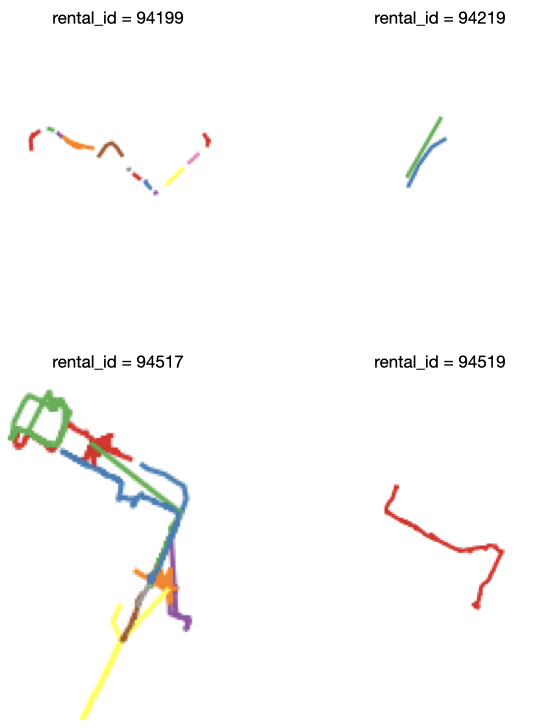
\includegraphics[width=\columnwidth]{timedelta-result}
		\caption{Timedelta heuristic line plot in details}
		\label{fig:timedelta-result}
	\end{figure}

	\begin{figure}[bt]
		\centering
		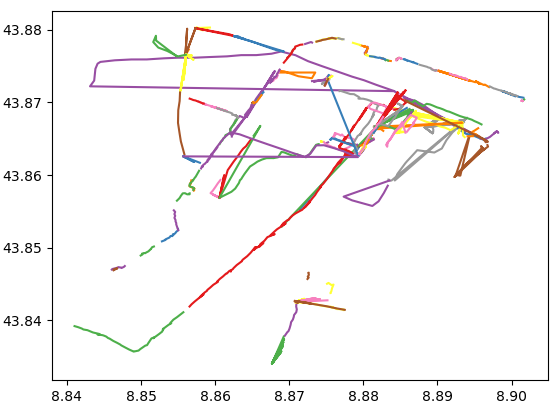
\includegraphics[width=\columnwidth]{timedelta-lineplot}
		\caption{Timedelta heuristic line plot in the entire city}
		\label{fig:timedelta-lineplot}
	\end{figure}

	\item \textit{spreddelta heuristic}: in figure \ref{fig:spreaddelta-result} you can see how the trajectories are clusterized in 3 main groups: wide area trajectories (green), medium area trajectories (blue) and small area trajectories (red). The trajectories showed in figure are grouped starting from the \textit{timedelta} division performed before. 
	
	\begin{figure}[bt]
		\centering
		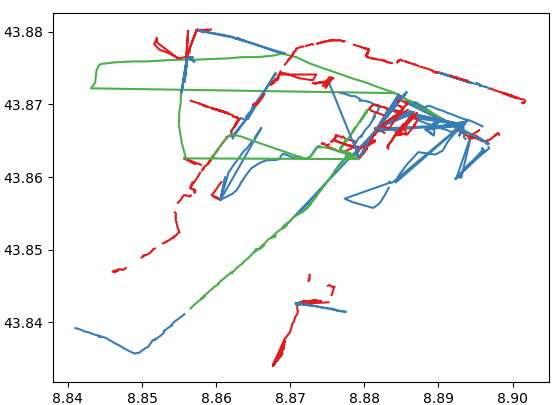
\includegraphics[width=\columnwidth]{spreaddelta-result}
		\caption{Spreaddelta heuristic line plot}
		\label{fig:spreaddelta-result}
	\end{figure}
	
	\item \textit{edgedelta heuristic}: in figure \ref{fig:edgedelta-result} you can see how the trajectories are clusterized in relation to the start and end positions of each trajectory generated by \textit{timedelta heuristic}. This heuristic performs some good results, because it is able to recognize the neighbours trajectories, but there are also some result not expected due to the problem of bimodal distribution.  
	
	\begin{figure}[bt]
		\centering
		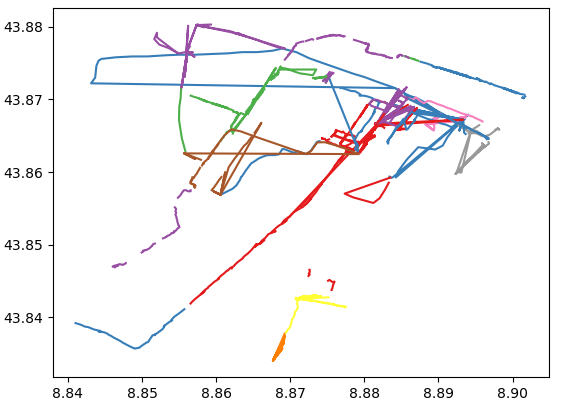
\includegraphics[width=\columnwidth]{edgedelta-result}
		\caption{Edgedelta heuristic line plot}
		\label{fig:edgedelta-result}
	\end{figure}
	
	\item \textit{coorddelta heuristic}: in figure \ref{fig:coorddelta-result} you can see the trajectories clusterized with both \textit{edgedelta} and \textit{spreaddelta} techniques. It shows the same issues of \textit{edgedelta heuristic}, but, with the \textit{spreaddelta heuristic} addition, the trajectories are even more selective, to the point of returning nearly to the initial trajectories. This heuristic can be useful only if you want a model that slightly clusterize the trajectories.
	
	\begin{figure}[bt]
		\centering
		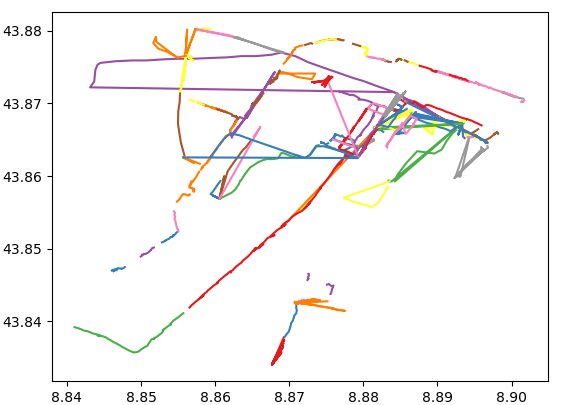
\includegraphics[width=\columnwidth]{coorddelta-result}
		\caption{Coorddelta heuristic line plot}
		\label{fig:coorddelta-result}
	\end{figure}

\end{itemize}

For clustering algorithms, in addition to graph analysis, I also use the \textit{Silhouette} validation. To evaluate the number of clusters for the algorithms that need it as parameter, I executed \textit{K-Means} for a number of cluster in a range from 1 to 30 and I calculated for each cluster number the \textit{WCSS error}. Then I plot the \textit{WCSS} graph and I used \textit{Elbow method} to choose the best value to use. As result of \textit{WCSS} graph, I chose to set 5 clusters. 

\begin{figure}[bt]
	\centering
	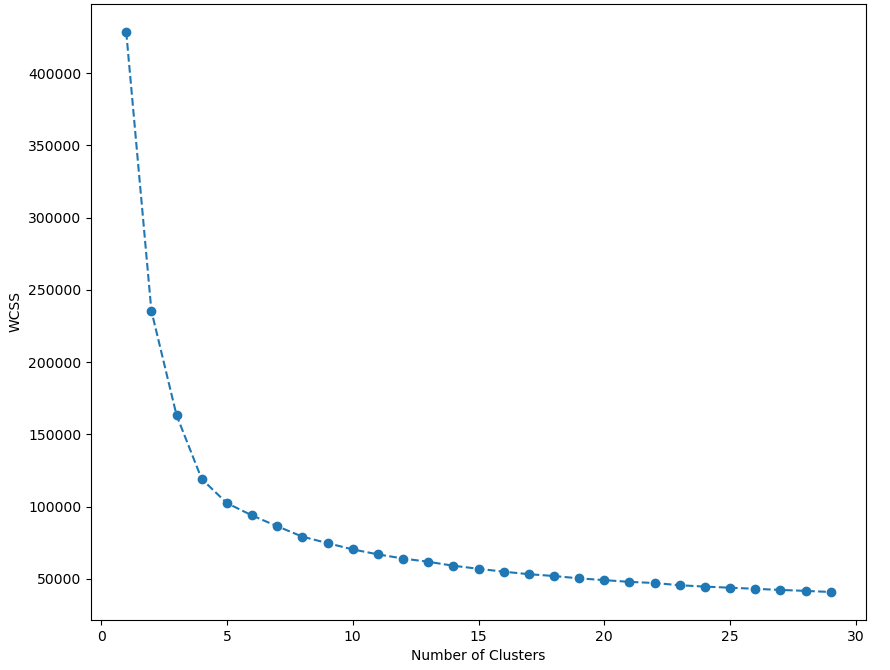
\includegraphics[width=\columnwidth]{wcss}
	\caption{Within Cluster Sum of Squares (WCSS) graph for Elbow method in range 1 to 30 with K-Means}
	\label{fig:wcss}
\end{figure}

All clustering techniques were performed on each city individually, in order to facilitate the algorithms. The results of clustering techniques are the following: 

\begin{itemize}
	\item \textit{Gaussian Mixture}: performs bad result \ref{fig:gaussian-mixture-line} and the silhouette validation confirms it.
	
	\begin{figure}[bt]
		\centering
		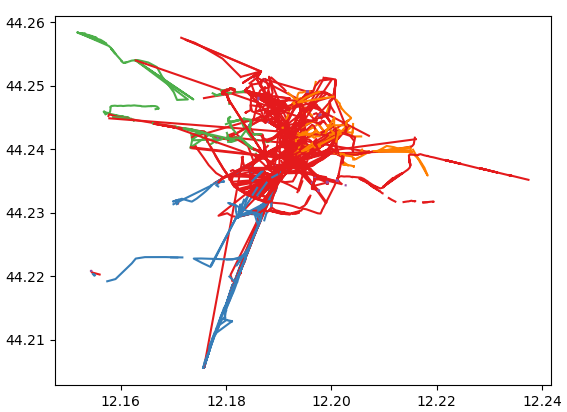
\includegraphics[width=\columnwidth]{gaussian-mixture-plot}
		\caption{Gaussian Mixture line plot with silhouette -0.02}
		\label{fig:gaussian-mixture-line}
	\end{figure}

	\item \textit{Mean Shift}: obtains the best result in terms of silhouette validation. The number of cluster generated is only 3 because \textit{Mean Shift}, at the end of algorithm, performs a pruning operation of similar centres, taking only the more significant. In general, for trajectory clustering, I would like to obtain more clusters, but this is also an alert that the number of clusters can't be really higher. 
	
	\begin{figure}[bt]
		\centering
		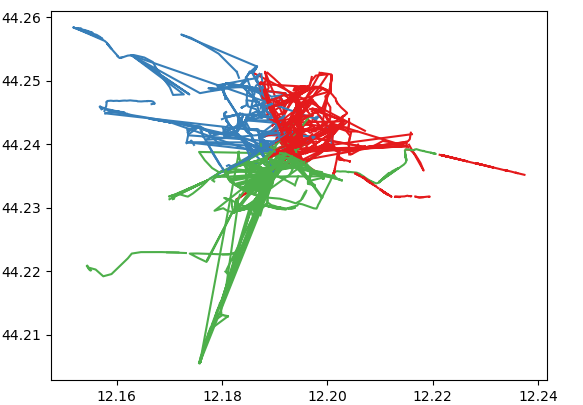
\includegraphics[width=\columnwidth]{mean-shift-plot}
		\caption{Mean Shift line plot with silhouette 0.40}
		\label{fig:mean-shift-line}
	\end{figure}

	\item \textit{Full Hierarchical Agglomerative}: worst both in silhouette validation term and representation term \ref{fig:full-agglomerative-line}, but the main issue of this technique is a huge memory cost. The dedrogram of this hierarchical algorithm is shown in the this figure \ref{fig:full-agglomerative-dendrogram}. 
	
	\begin{figure}[bt]
		\centering
		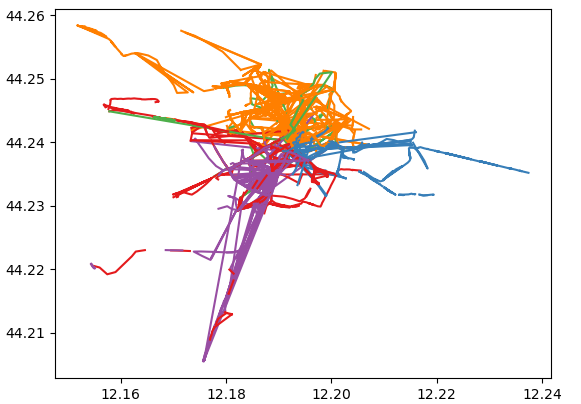
\includegraphics[width=\columnwidth]{full-agglomerative-plot}
		\caption{Full Hierarchical Agglomerative line plot with silhouette 0.16}
		\label{fig:full-agglomerative-line}
	\end{figure}

	\begin{figure}[bt]
		\centering
		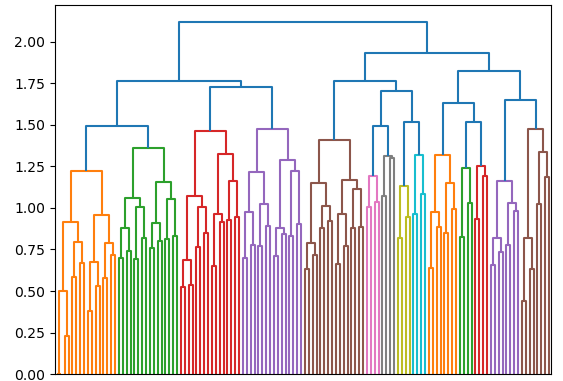
\includegraphics[width=\columnwidth]{full-agglomerative-dendrogram}
		\caption{Full Hierarchical Agglomerative dendrogram up to level 5 of merge}
		\label{fig:full-agglomerative-dendrogram}
	\end{figure}

	\item \textit{Ward Hierarchical Agglomerative}: performs well because it tries to group the centre of the city. It is really similar to \textit{K-Means}, it is not as accurate as \textit{K-Means}, but the main problem, like the \textit{Full} version of this technique, is the huge memory cost. The dedrogram of this hierarchical algorithm is shown in the this figure \ref{fig:ward-agglomerative-dendrogram}. 
	
	\begin{figure}[bt]
		\centering
		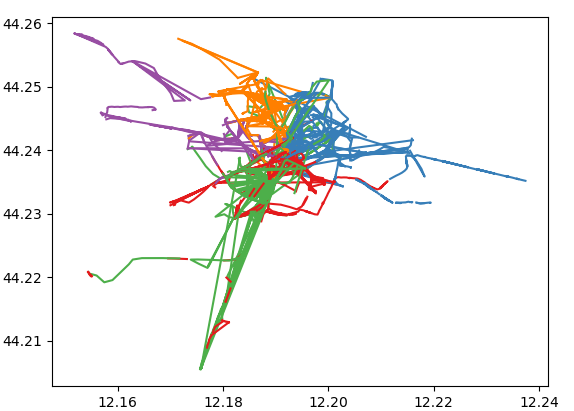
\includegraphics[width=\columnwidth]{ward-agglomerative-plot}
		\caption{Ward Hierarchical Agglomerative line plot with silhouette 0.28}
		\label{fig:ward-agglomerative-line}
	\end{figure}
	
	\begin{figure}[bt]
		\centering
		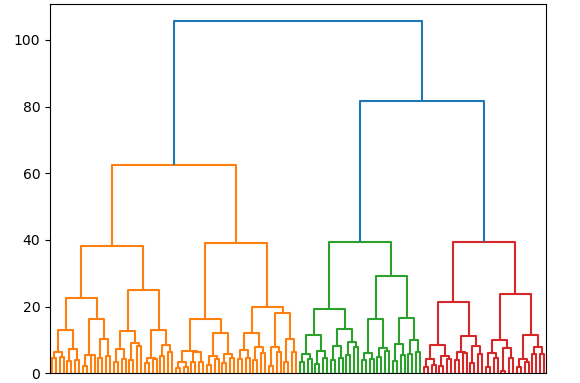
\includegraphics[width=\columnwidth]{ward-agglomerative-dendrogram}
		\caption{Ward Hierarchical Agglomerative dendrogram up to level 5 of merge}
		\label{fig:ward-agglomerative-dendrogram}
	\end{figure}

	\item \textit{K-Means}: it is the simplest algorithm but maybe the one that produces the best results. Even if it uses a distance metric to calculate the clusters, it performs very well not only in terms of plot representation, but also in silhouette value. In addition, it is really fast and cheap in memory. The main problem of this clustering result is the mixture of clusters in the city centre, that creates uncertainty.
	
	\begin{figure}[bt]
		\centering
		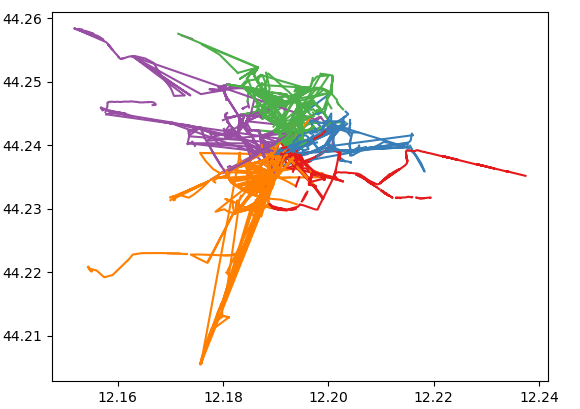
\includegraphics[width=\columnwidth]{k-means-plot}
		\caption{K-Means line plot with silhouette 0.352}
		\label{fig:k-means-line}
	\end{figure}
	
\end{itemize}